% AA-66
\chapter{Twierdzenie Weyla i operator Casimira}
\label{aa:ch:weyl-complete-reducibility}

W AA-65 uzyskaliśmy jednoznaczność reprezentacji nieprzywiedlnej o ustalonej wadze najwyższej. Nie wynika z niej jeszcze, że każda reprezentacja jest sumą prostą reprezentacji nieprzywiedlnych. Istotą tego rozdziału jest wykazanie, że każdy podmoduł reprezentacji skończenie wymiarowej algebry półprostej ma niezmiennicze dopełnienie. Dowód wykorzystuje formę śladu i nie wymaga klasyfikacji reprezentacji.

\section{Operator Casimira}

\begin{lemat}
\label{aa:lem:lie-faithful-trace}
Niech $K$ będzie algebraicznie domkniętym ciałem charakterystyki zero, $\mathfrak g$ skończenie wymiarową półprostą algebrą Liego nad $K$, a $\rho:\mathfrak g\to\mathfrak{gl}(V)$ wierną reprezentacją w skończenie wymiarowej przestrzeni $V$. Forma $B(x,y)=\operatorname{tr}_V(\rho(x)\rho(y))$ jest niezdegenerowana.
\end{lemat}
\begin{proof}
Forma $B$ jest symetryczna i niezmiennicza na mocy Stwierdzenia~\ref{aa:prop:killing-properties}. Jej jądro $\mathfrak a$ jest ideałem z Lematu~\ref{aa:lem:lie-orthogonal-ideals}. Dla $x\in[\mathfrak a,\mathfrak a]$ i $y\in\mathfrak a$ mamy $B(x,y)=0$. Kryterium Cartana dla podalgebr macierzy (Twierdzenie~\ref{aa:tw:cartan-linear}) zastosowane do $\rho(\mathfrak a)$ daje rozwiązalność $\rho(\mathfrak a)$. Wierność reprezentacji oznacza, że $\mathfrak a$ jest izomorficzna z $\rho(\mathfrak a)$, więc $\mathfrak a$ jest rozwiązalnym ideałem algebry półprostej. Zatem $\mathfrak a=0$.
\end{proof}

\begin{definicja}
\label{aa:def:lie-casimir}
Niech $\mathfrak g$ będzie skończenie wymiarową algebrą Liego nad ciałem $K$, $B$ symetryczną niezdegenerowaną niezmienniczą formą dwuliniową na $\mathfrak g$, a $\rho:\mathfrak g\to\mathfrak{gl}(V)$ reprezentacją. Dla bazy $(x_i)_{i=1}^d$ algebry $\mathfrak g$, gdzie $d=\dim\mathfrak g$, niech $(y_i)_{i=1}^d$ będzie bazą sprzężoną względem $B$, czyli $B(x_i,y_j)=\delta_{ij}$. Operatorem Casimira związanym z $B$ na $V$ nazywamy
\[
 C_B=\sum_{i=1}^d\rho(x_i)\rho(y_i).
\]
\end{definicja}

\begin{lemat}
\label{aa:lem:lie-casimir-identity}
Niech $\mathfrak g$ będzie skończenie wymiarową algebrą Liego nad ciałem $K$, $B$ symetryczną niezdegenerowaną niezmienniczą formą dwuliniową na $\mathfrak g$, $(x_i)_{i=1}^d$ bazą $\mathfrak g$, $(y_i)_{i=1}^d$ bazą sprzężoną względem $B$, a $\rho:\mathfrak g\to\mathfrak{gl}(V)$ reprezentacją. Wówczas element $\Omega_B=\sum_i x_i\otimes y_i\in\mathfrak g\otimes_K\mathfrak g$ nie zależy od wyboru bazy i dla każdego $z\in\mathfrak g$ zachodzi
\[
 \sum_i [z,x_i]\otimes y_i+x_i\otimes[z,y_i]=0.
\]
W szczególności $C_B$ nie zależy od wyboru bazy i komutuje z każdym $\rho(z)$.
\end{lemat}
\begin{proof}
Izomorfizm $\mathfrak g\otimes_K\mathfrak g\to\operatorname{End}_K(\mathfrak g)$ określony na tensorach prostych wzorem $u\otimes v\mapsto (t\mapsto B(v,t)u)$ wynika z niezdegenerowania $B$ i standardowego izomorfizmu z przestrzenią endomorfizmów. Obraz $\Omega_B$ jest identycznością, ponieważ $t=\sum_i B(y_i,t)x_i$. Stąd niezależność od bazy.

Obraz lewej strony to operator wysyłający $t$ na
\[
 \sum_i B(y_i,t)[z,x_i]+\sum_i B([z,y_i],t)x_i
 =[z,t]-\sum_i B(y_i,[z,t])x_i=0.
\]
Użyliśmy niezmienniczości formy w postaci $B([z,y],t)=-B(y,[z,t])$. Iniektywność izomorfizmu daje żądaną tożsamość. Stosując liniowe odwzorowanie $u\otimes v\mapsto\rho(u)\rho(v)$, otrzymujemy
\[
 [\rho(z),C_B]=\sum_i\rho([z,x_i])\rho(y_i)+
 \rho(x_i)\rho([z,y_i])=0.
\]
Niezależność $C_B$ wynika z niezależności $\Omega_B$.
\end{proof}

\section{Pierwszy lemat Whiteheada}

\begin{definicja}
\label{aa:def:lie-one-cocycle}
Niech $\mathfrak g$ będzie algebrą Liego nad ciałem $K$, a $M$ jej modułem. Liniowe odwzorowanie $f:\mathfrak g\to M$ nazywamy $1$-kocyklem, jeśli
\[
 f([x,y])=xf(y)-yf(x)\qquad(x,y\in\mathfrak g).
\]
Jeśli istnieje $m\in M$ takie, że $f(x)=xm$ dla każdego $x\in\mathfrak g$, nazywamy $f$ $1$-kobrzegiem.
\end{definicja}

Każdy $1$-kobrzeg jest $1$-kocyklem, ponieważ $[x,y]m=x(ym)-y(xm)$. Przestrzeń ilorazowa $1$-kocykli przez $1$-kobrzegi jest oznaczana przez $H^1(\mathfrak g,M)$.

\begin{twierdzenie}[Pierwszy lemat Whiteheada]
\label{aa:tw:lie-whitehead-one}
Niech $K$ będzie algebraicznie domkniętym ciałem charakterystyki zero, $\mathfrak g$ skończenie wymiarową półprostą algebrą Liego nad $K$, a $M$ skończenie wymiarowym $\mathfrak g$-modułem. Każdy $1$-kocykl $f:\mathfrak g\to M$ jest $1$-kobrzegiem, czyli $H^1(\mathfrak g,M)=0$.
\end{twierdzenie}
\begin{proof}
Najpierw załóżmy, że $M$ jest niezerowy i nieprzywiedlny. Jeśli działanie $\mathfrak g$ na $M$ jest trywialne, warunek kocyklu daje $f([\mathfrak g,\mathfrak g])=0$. Ponieważ $\mathfrak g=[\mathfrak g,\mathfrak g]$ na mocy Wniosku~\ref{aa:cor:semisimple-perfect}, otrzymujemy $f=0$.

W przypadku działania nietrywialnego oznaczmy przez $\mathfrak a$ jądro reprezentacji. Z Twierdzenia~\ref{aa:tw:semisimple-decomposition} mamy rozkład $\mathfrak g=\mathfrak a\oplus\mathfrak l$ na komutujące ideały, które są półproste: ideał rozwiązalny jednego składnika byłby także ideałem całej $\mathfrak g$. Przy tym $\mathfrak l\ne0$. Dla $x,y\in\mathfrak a$ warunek kocyklu daje $f([x,y])=0$, a półprostota $\mathfrak a$ daje $[\mathfrak a,\mathfrak a]=\mathfrak a$, więc $f|_{\mathfrak a}=0$. Wystarczy zatem rozważyć ograniczenie $f$ do $\mathfrak l$. Moduł $M$ pozostaje nieprzywiedlny względem $\mathfrak l$, ponieważ $\mathfrak a$ działa zerowo, a reprezentacja $\mathfrak l$ jest wierna.

Na $\mathfrak l$ wybieramy formę $B(x,y)=\operatorname{tr}_M(\rho(x)\rho(y))$, niezdegenerowaną na mocy Lematu~\ref{aa:lem:lie-faithful-trace}. Operator $C_B$ komutuje z działaniem $\mathfrak l$. Ponieważ $K$ jest algebraicznie domknięte, $C_B$ ma wartość własną $c$, a jej niezerowa przestrzeń własna jest podmodułem. Nieprzywiedlność daje $C_B=cI_M$. Dla baz sprzężonych względem $B$ mamy
\[
 c\dim M=\operatorname{tr}_M C_B
 =\sum_i B(x_i,y_i)=\dim\mathfrak l.
\]
Oba wymiary są dodatnie, więc $c\ne0$ w charakterystyce zero. Nie twierdzimy, że operator Casimira względem dowolnej formy niezmienniczej musi mieć niezerową wartość własną; wybór formy śladu jest tu istotny.

Niech $u=\sum_i x_i f(y_i)\in M$, gdzie bazy dotyczą $\mathfrak l$. Dla $z\in\mathfrak l$ mamy
\begin{align*}
 zu&=\sum_i [z,x_i]f(y_i)+x_i(zf(y_i))\\
   &=\sum_i [z,x_i]f(y_i)+x_i f([z,y_i])
       +\sum_i x_i y_i f(z)\\
   &= C_B f(z)=cf(z).
\end{align*}
W drugiej równości użyto warunku kocyklu, a w trzeciej zastosowano do tożsamości z Lematu~\ref{aa:lem:lie-casimir-identity} liniowe odwzorowanie $x\otimes y\mapsto xf(y)$. Zatem $f(z)=z(c^{-1}u)$. Dla $z\in\mathfrak a$ obie strony są zerowe, więc wzór obowiązuje na całej $\mathfrak g$.

Przechodzimy do dowolnego $M$, indukując po jego wymiarze. Dla $M=0$ teza jest oczywista. Przypadek nieprzywiedlny już udowodniliśmy. W przeciwnym razie wybierzmy niezerowy właściwy podmoduł $N\subset M$ i niech $q:M\to M/N$ będzie rzutem ilorazowym. Odwzorowanie $q\circ f$ jest kocyklem, gdyż $q$ jest homomorfizmem modułów. Z indukcji istnieje $\bar m\in M/N$ takie, że $qf(x)=x\bar m$ dla wszystkich $x$. Wybierzmy $m\in M$ z $q(m)=\bar m$. Wówczas $f_0(x)=f(x)-xm$ należy do $N$ i jest kocyklem z wartościami w $N$, jako różnica dwóch kocykli. Ponownie z indukcji istnieje $n\in N$ takie, że $f_0(x)=xn$. Zatem $f(x)=x(m+n)$, co kończy dowód.
\end{proof}

\section{Rozszczepianie rozszerzeń modułów}

\begin{twierdzenie}[Twierdzenie Weyla]
\label{aa:tw:lie-weyl-complete-reducibility}
Niech $K$ będzie ciałem charakterystyki zero, $\mathfrak g$ skończenie wymiarową półprostą algebrą Liego nad $K$, a $V$ skończenie wymiarowym $\mathfrak g$-modułem. Każdy podmoduł $U\subset V$ ma dopełnienie będące podmodułem. W szczególności $V$ jest sumą prostą skończenie wielu modułów nieprzywiedlnych.
\end{twierdzenie}
\begin{proof}
Najpierw załóżmy, że $K$ jest algebraicznie domknięte. Niech $W=V/U$, $q:V\to W$ będzie rzutem ilorazowym, a $s:W\to V$ liniowym przekrojem $q$ (czyli $qs=I_W$), otrzymanym przez podniesienie bazy $W$ do $V$. Nie zakładamy, że $s$ jest homomorfizmem modułów.

Na $M=\operatorname{Hom}_K(W,U)$ definiujemy działanie $(xT)(w)=x(Tw)-T(xw)$. Jest to reprezentacja: rozwijając $x(yT)-y(xT)$, składniki mieszane redukują się, a pozostaje $[x,y]T-T[x,y]$, gdzie pierwszy nawias działa na $U$, drugi na $W$. Analogiczne działanie mamy na $\operatorname{Hom}_K(W,V)$.

Dla $x\in\mathfrak g$ definiujemy $f(x)=xs-sx$, czyli $f(x)(w)=x(s(w))-s(xw)$. Ponieważ $q$ jest homomorfizmem modułów, $qf(x)(w)=xw-xw=0$, więc $f(x)$ ma wartości w $U$. W języku reprezentacji na przestrzeni homomorfizmów $f(x)=x\cdot s$, a z tożsamości reprezentacji $f([x,y])=x\cdot f(y)-y\cdot f(x)$. Jest to zatem kocykl z wartościami w $M$.

Na mocy Twierdzenia~\ref{aa:tw:lie-whitehead-one} istnieje $T\in M$ takie, że $f(x)=xT$ dla każdego $x$. Traktujemy $T$ jako odwzorowanie do $V$ przez inkluzję $U\subset V$. Wtedy $s'=s-T$ spełnia $qs'=I_W$, ponieważ $qT=0$, oraz $x\cdot s'=f(x)-xT=0$. Oznacza to, że $s'$ jest homomorfizmem modułów. Podprzestrzeń $U'=s'(W)$ jest podmodułem; jeśli $s'(w)\in U$, to $w=qs'(w)=0$. Każdy $v\in V$ ma rozkład $v=(v-s'q(v))+s'q(v)$, gdzie pierwszy składnik należy do $U$. Stąd $V=U\oplus U'$.

Dla dowolnego ciała $K$ charakterystyki zero przechodzimy do domknięcia algebraicznego $\overline K$. Forma Killinga $\mathfrak g$ jest niezdegenerowana na mocy Twierdzenia~\ref{aa:tw:cartan-semisimple}. Po rozszerzeniu skalarów jej macierz w rozszerzonej bazie pozostaje ta sama, więc algebra $\mathfrak g_{\overline K}$ jest półprosta na mocy tego samego kryterium. Reprezentacja i podmoduł rozszerzają się do $V_{\overline K},U_{\overline K}$. Z już udowodnionego przypadku istnieje rzut $P_{\overline K}:V_{\overline K}\to U_{\overline K}$, który jest homomorfizmem modułów i na $U_{\overline K}$ jest identycznością.

Warunki na nieznane odwzorowanie $P:V\to U$,
\[
 P|_U=I_U,\qquad P\rho_V(x)=\rho_U(x)P\quad(x\in\mathfrak g),
\]
tworzą skończony układ liniowych równań nad $K$ (wystarczy wziąć bazę $\mathfrak g$). Układ ma rozwiązanie nad $\overline K$, zatem ma rozwiązanie nad $K$: eliminacja Gaussa nad $K$ nie może dać sprzecznego wiersza, gdyż ten sam wiersz byłby sprzeczny po rozszerzeniu skalarów. Dla tak otrzymanego $P$ jądro jest podmodułem, a $v=(v-Pv)+Pv$ daje rozkład $V=\ker P\oplus U$.

Wreszcie indukcja po wymiarze $V$ daje rozkład na moduły nieprzywiedlne. Dla $V=0$ przyjmujemy pustą sumę. Dla $V\ne0$ wybieramy niezerowy podmoduł najmniejszego wymiaru, który jest nieprzywiedlny. Jego dopełnienie ma mniejszy wymiar, więc stosujemy do niego indukcję.
\end{proof}

\begin{center}
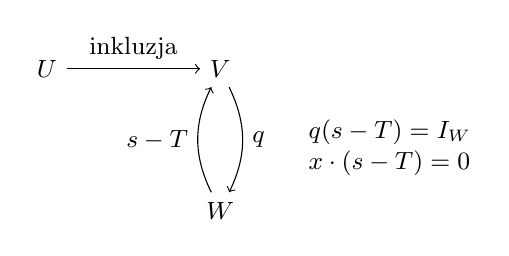
\begin{tikzpicture}[every node/.style={font=\small}]
\node (w) at (0,0) {$W$};
\node (v) at (0,1.8) {$V$};
\node (u) at (-2.2,1.8) {$U$};
\draw[->] (u)--node[above] {inkluzja} (v);
\draw[->] (v) to[bend left=26] node[right] {$q$} (w);
\draw[->] (w) to[bend left=26] node[left] {$s-T$} (v);
\node[align=left,anchor=west] at (1.0,.8) {$q(s-T)=I_W$\\$x\cdot(s-T)=0$};
\end{tikzpicture}

\small Korekta liniowego przekroju daje przekrój będący homomorfizmem modułów.
\end{center}

\begin{przyklad}[Iloczyn tensorowy reprezentacji naturalnej i sprzężonej]
\label{aa:prz:weyl-endomorphisms}
Niech $K$ będzie ciałem charakterystyki zero i $n\ge2$. Dla naturalnej reprezentacji $V=K^n$ algebry $\mathfrak{sl}_n(K)$ identyfikujemy $V\otimes_K V^*$ z $\operatorname{End}_K(V)$ przez $v\otimes\varphi\mapsto(w\mapsto\varphi(w)v)$. Działanie na endomorfizmach to komutator $xA-Ax$: wynika to z działania sprzężonego $x\varphi=-\varphi\circ x$. Podmoduł macierzy skalarnych $KI_n$ ma niezmiennicze dopełnienie $\mathfrak{sl}_n(K)$, ponieważ ślad komutatora jest zerowy i
\[
 A=\frac{\operatorname{tr}A}{n}I_n+
       \left(A-\frac{\operatorname{tr}A}{n}I_n\right).
\]
Przykład pokazuje konkretny rozkład na podmoduły, którego istnienie gwarantuje twierdzenie Weyla.
\end{przyklad}

\begin{przyklad}[Konieczność założenia półprostoty]
\label{aa:prz:weyl-nonsemisimple}
Niech $\mathfrak g=Kx$ będzie jednowymiarową abelową algebrą Liego nad ciałem charakterystyki zero. Na przestrzeni $V=Ke_1+Ke_2$ definiujemy $xe_1=0$, $xe_2=e_1$. Jest to reprezentacja, gdyż algebra jest generowana przez jeden element i jego komutator z samym sobą jest zerowy. Podmoduł $U=Ke_1$ nie ma niezmienniczego dopełnienia. Każda dopełniająca prosta jest rozpięta przez $e_2+ae_1$ dla pewnego $a\in K$, a obraz tego wektora przez $x$ jest równy $e_1$, który do tej prostej nie należy. Tutaj $W=V/U$ jest modułem trywialnym, podobnie jak $U$. Kocykiel $f(x)(e_2+U)=e_1$ jest niezerowy, ale każdy kobrzeg w $\operatorname{Hom}_K(W,U)$ jest zerowy, gdyż działanie jest trywialne. Wyjaśnia to dokładnie, dlaczego dowód rozszczepiania przestaje działać.
\end{przyklad}
